\section{Model Details}
\label{app:models}

\subsection{Constellation Experiments}
\label{app:constellation_model}
The \gls{CCAu} uses a four-layer Set Transformer as its encoder.
Every layer has four attention heads, 128 hidden units per head, and is followed by layer norm \citep{Ba2016layern}.
The encoder outputs three 32-dimensional vectors---one for each object capsule.
The decoder uses a separate neural net for each object capsule to predict all parameters used to model its points: this includes four candidate part predictions per capsule for a total of 12 candidates.
In this experiment, each object$\rightarrow$part relationship \gls{OP} is just a 2-D offset in the object's frame of reference (instead of a $3\times3$ matrix) and it is affine transformed by the corresponding \gls{OV} matrix to predict the 2-D point.

\subsection{Image Experiments}

We use a convolutional encoder for part capsules and a set transformer encoder \citep{Lee2019set} for object capsules.
Decoding from object capsule to part capsules is done with \glspl{MLP}, while the input image is reconstructed with affine-transformed learned templates.
Details of the architectures we used are available in \Cref{tab:arch}.
\begin{center}
\centering
    \captionof{table}{
        Architecture details. \textsc{S} in the last column means that the entry is the same as for \textsc{svhn}.
    }
    \label{tab:arch}
    \small
    \begin{tabular}{@{}lllll@{}}
        Dataset & Constellation & \textsc{mnist} & \textsc{svhn} & \textsc{cifar10} \\
        \midrule
        num templates & N/A & 24 & 24 & 32\\
        template size & N/A & $11\times11$ & $14\times14$ & \textsc{s}\\
        num capsules & 3 & 24 & 32 & 64\\
        part \textsc{cnn} & N/A & 2x(128:2)-2x(128:1) & 2x(128:1)-2x(128:2) & \textsc{s} \\
        set transformer & 4x(4-128)-32  & 3x(1-16)-256 & 3x(2-64)-128 & \textsc{s}
\end{tabular}
\end{center}

We use ReLu nonlinearities except for presence probabilities, for which we use sigmoids.
(128:2) for a \gls{CNN} means 128 channels with a stride of two.
All kernels are $3\times3$.
For set transformer (1-16)-256 means one attention head, 16 hidden units and 256 output units; it uses layer normalization \citep{Ba2016layern} as in the original paper \citep{Lee2019set} but no dropout. All experiments (apart from constellations) used 16 special features per part capsule.

For \textsc{svhn} and \textsc{cifar10}, we use normalized sobel-filtered images as the target of the reconstruction to emphasize the shape importance. \Cref{fig:svhn_recons} in \Cref{app:recs} shows examples of \textsc{svhn} and \textsc{cifar10} reconstruction.
The filtering procedure is as follows:
1) apply sobel filtering, 2) subtract the median color, 3) take the absolute value of the image, 4) normalize for image values to be $\in \interval{0, 1}$.

All models are trained with the RMSProp optimizer \citep{Tieleman2012rms} $\mathrm{momentum}=.9$ and $\epsilon = \left(10 * \mathrm{batch\_size}\right)^{-2}$.
Batch size is 64 for constellations and 128 for all other datasets.
The learning rate was equal to $10^{-5}$ for \textsc{mnist} and constellation experiments (without any decay), while we run a hyperparameter search for \textsc{svhn} and \textsc{cifar10}: we searched learning rates in the range of $5*10^{-5}$ to $5*10^{-4}$ and exponential learning rate decay of 0.96 every $10^3$ or $3*10^3$ weight updates. Learning rate of $10^{-4}$ was selected for both \textsc{svhn} and \textsc{cifar10}, the decay steps was $10^3$ for \textsc{svhn} and $3*10^3$ for \textsc{cifar10}.
The $\textsc{lin-pred}$ accuracy on a validation set is used as a proxy to select the best hyperparameters---including weights on different losses, reported in \Cref{tab:hparams}.
Models were trained for up to $3*10^5$ iterations on single Tesla V100 GPUs, which took 40 minutes for constellation experiments and less than a day for \textsc{cifar10}.

\begin{center}
\centering
    \captionof{table}{
        Loss weights values. The \textit{within} and \textit{between} quantifiers in sparsity losses corresponds to different terms of \Cref{eq:prior_sparsity,eq:posterior_sparsity}.
    }
    \label{tab:hparams}
    \small
    \begin{tabular}{@{}lllll@{}}
        Dataset & Constellation & \textsc{mnist} & \textsc{svhn} & \textsc{cifar10} \\
        \midrule
        part ll weight & 1 & 1 & 2.56 & 2.075 \\
        image ll weight & N/A & 1 & 1 & 1\\
        prior within sparsity & 1  & 1 & 0.22 & 0.17 \\
        prior between sparsity & 1  & 1 & 0.1 & 0.1 \\
        posterior within sparsity & 0 & 10 & 8.62 & 1.39 \\
        posterior between sparsity & 0 & 10 & 0.26 & 7.32 \\
        too-few-active-capsules & 10 & 0 & 0 & 0
\end{tabular}
\end{center}

\section{Reconstructions}
\label{app:recs}
\begin{center}
\begin{tabular}{ >{\centering\arraybackslash}m{.1\linewidth} >{\centering\arraybackslash}m{.85\linewidth}}
SVHN & 
    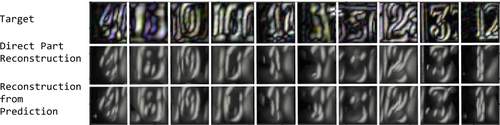
\includegraphics[width=\linewidth]{figures/SCA/svhn_recons.png}
\\
CIFAR10 & 
    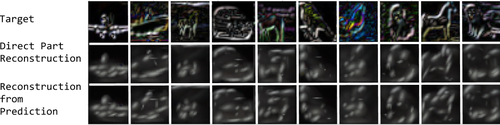
\includegraphics[width=\linewidth]{figures/SCA/cifar_recons.png}
    \end{tabular}
    \captionof{figure}{10 Sample SVHN and Cifar10 reconstructions. First row shows Sobel filtered target image. Second row shows the reconstruction from Part Capsule Layer directly. Third row shows the reconstruction if we use the object predictions for the Part poses instead of Part poses themselves for reconstruction. The templates in this model has the same number of channels as the image, but they have converged to black and white templates and the reconstruction do not have color diversity. The \gls{SCAu} model is trained completely unsupervised but the reconstructions tend to focus on the center digit in SVHN and filter the rest of the clutter. }
    \label{fig:svhn_recons}
\end{center}

